\documentclass[UTF8,openany,10pt]{ctexrep}
\usepackage[a4paper,top=20mm,bottom=21mm,left=22mm,right=22mm,headheight=15pt]{geometry}
\usepackage{booktabs,longtable,tabularx,array,multirow,makecell}
\usepackage{graphicx,subcaption,float,placeins}
\usepackage{amsmath,amssymb}
\usepackage{siunitx}
\usepackage{xcolor}
\usepackage{tikz}
\usetikzlibrary{arrows.meta,positioning,fit,shapes.geometric,calc}
\usepackage{pgfplots}
\pgfplotsset{compat=1.18}
\usepackage{hyperref}
\usepackage[nameinlink,noabbrev]{cleveref}
\usepackage{xurl}
\usepackage{fancyhdr}
\usepackage{enumitem}
\usepackage{setspace}
\usepackage{microtype}
\usepackage{caption}
\usepackage{titlesec}

\definecolor{ReportNavy}{HTML}{142B4A}
\definecolor{ReportBlue}{HTML}{2474B5}
\definecolor{ReportTeal}{HTML}{168B83}
\definecolor{ReportAmber}{HTML}{E69F35}
\definecolor{ReportRed}{HTML}{C6534C}
\definecolor{ReportGreen}{HTML}{4C956C}
\definecolor{ReportGray}{HTML}{667085}
\definecolor{ReportLight}{HTML}{F2F6F8}

\hypersetup{
  colorlinks=true,
  linkcolor=ReportBlue,
  urlcolor=ReportBlue,
  citecolor=ReportBlue,
  pdftitle={ALOHA机器人拧瓶盖项目现阶段技术报告},
  pdfsubject={第一年度工作总结与下一年度计划},
  pdfauthor={待填写}
}
\graphicspath{{figures/}}
\setlength{\emergencystretch}{2.5em}
\setlength{\parindent}{2em}
\setlength{\parskip}{0.25em}
\setstretch{1.17}
\setlist{topsep=3pt,itemsep=2pt,parsep=0pt,leftmargin=2em}
\captionsetup{font=small,labelfont=bf,labelsep=quad}
\renewcommand{\arraystretch}{1.22}
\setlength{\tabcolsep}{5pt}
\setcounter{tocdepth}{2}
\setcounter{secnumdepth}{2}

\titleformat{\chapter}[display]
  {\bfseries\color{ReportNavy}}
  {\filleft\Large 第\thechapter 章}
  {0.3ex}
  {\titlerule\vspace{0.8ex}\Huge}
\titleformat{\section}{\Large\bfseries\color{ReportNavy}}{\thesection}{0.7em}{}
\titleformat{\subsection}{\large\bfseries\color{ReportBlue}}{\thesubsection}{0.7em}{}

\pagestyle{fancy}
\fancyhf{}
\fancyhead[L]{\small ALOHA 机器人拧瓶盖项目现阶段技术报告}
\fancyhead[R]{\small\color{ReportGray}\leftmark}
\fancyfoot[C]{\color{ReportGray}\thepage}
\renewcommand{\headrulewidth}{0.3pt}

\newcommand{\ev}[1]{\textcolor{ReportBlue}{\textsuperscript{[#1]}}}
\newcommand{\plain}[1]{\par\smallskip\noindent
  \colorbox{ReportLight}{\parbox{\dimexpr\linewidth-2\fboxsep}{\textbf{先说人话：}#1}}\par\smallskip}
\newcommand{\limitbox}[1]{\par\smallskip\noindent
  \fcolorbox{ReportAmber}{white}{\parbox{\dimexpr\linewidth-2\fboxsep-2\fboxrule}{\textbf{\color{ReportAmber}证据边界：}#1}}\par\smallskip}
\newcommand{\resultbox}[1]{\par\smallskip\noindent
  \fcolorbox{ReportGreen}{white}{\parbox{\dimexpr\linewidth-2\fboxsep-2\fboxrule}{\textbf{\color{ReportGreen}本阶段结论：}#1}}\par\smallskip}
\newcommand{\missing}{\textcolor{ReportRed}{当前证据中未找到直接记录}}
\newcommand{\figfull}[3][0.94\textwidth]{
  \begin{figure}[tbp]
    \centering
    \includegraphics[width=#1]{#2}
    \caption{#3}
  \end{figure}
}

\begin{document}
\begin{titlepage}
\thispagestyle{empty}
\begin{tikzpicture}[remember picture,overlay]
  \fill[ReportNavy] (current page.north west) rectangle ([yshift=-44mm]current page.north east);
  \fill[ReportTeal] ([yshift=-44mm]current page.north west) rectangle ([yshift=-47mm]current page.north east);
  \fill[ReportLight] (current page.south west) rectangle ([yshift=20mm]current page.south east);
\end{tikzpicture}
\vspace*{8mm}
{\color{white}\Large 第一年度工作总结与现阶段技术评审\par}
\vspace{11mm}
{\color{white}\fontsize{28}{34}\selectfont\bfseries
ALOHA 机器人拧瓶盖项目\\[2mm]现阶段技术报告\par}
\vspace{7mm}
\begin{center}
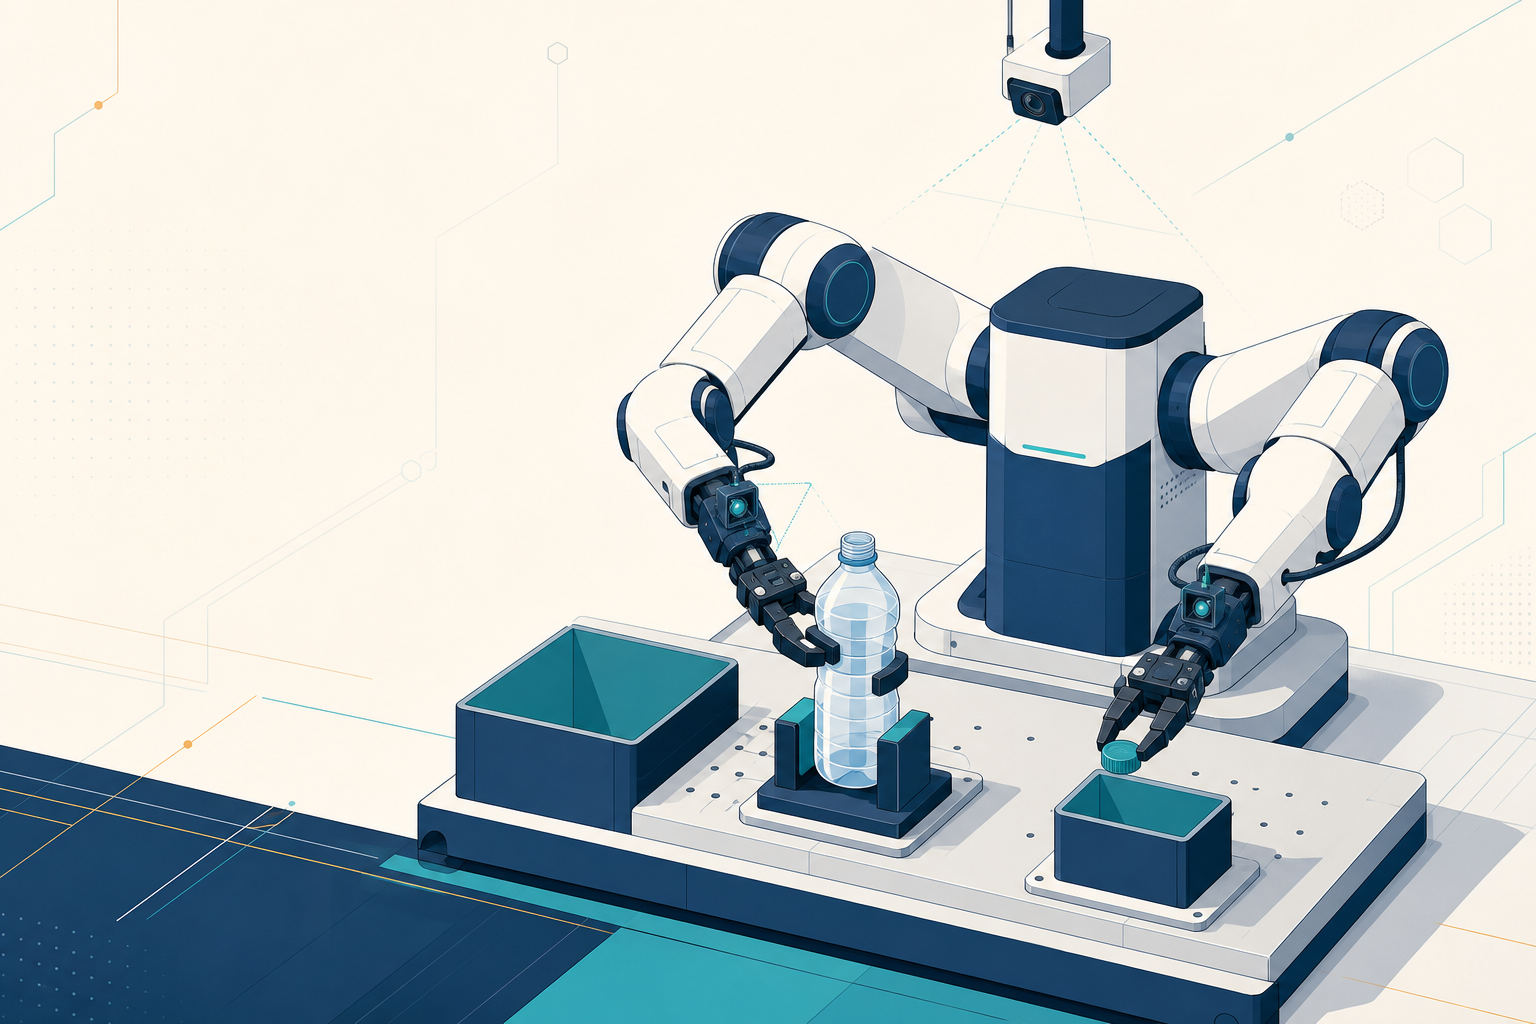
\includegraphics[width=.88\textwidth,height=.28\textheight,keepaspectratio]{cover_concept.png}

{\footnotesize\color{ReportGray}封面为任务概念示意图，不是实验照片。}
\end{center}
\vspace{4mm}
\begin{tabularx}{\textwidth}{>{\bfseries\color{ReportNavy}}p{32mm}X}
项目阶段 & 第一年工作总结与下一年度工作设计\\
正式部署模型 & 2026年5月训练、现场采用第19,000步保存版本\\
事实源版本 & 主仓库审计提交：\texttt{c90f1854}（完整编号见内部审计）\\
报告日期 & 2026年7月30日\\
报告版本 & v2.0（无演示视频、证据分级版）\\
作者 & \underline{\hspace{75mm}}\\
\end{tabularx}
\vspace{3mm}
{\small\color{ReportGray}用途：项目汇报、内部技术评审、后续论文材料整理\par}
\end{titlepage}

\pagenumbering{Roman}
\chapter*{摘要}
\addcontentsline{toc}{chapter}{摘要}

本项目面向废塑料瓶分拣场景，使用 ALOHA 双臂机器人学习一个完整长流程：左侧工作臂从散乱瓶堆中取瓶并稳定瓶身，右侧工作臂抓住瓶盖并旋下；随后左臂将瓶身投入一个回收盒，右臂将瓶盖投入另一个回收盒。任务同时包含随机目标发现、双臂协作、精细接触、连续旋转、物体分离和分类投放，比“一次抓起一个物体”明显更复杂。

第一年度已经形成从专用采集软件、数据编辑中心、数据版本发布、模型训练到机器人连续运行的完整工程闭环。数据平台现有 51 个有效 ALOHA 项目、2,413 条轨迹、2,907,804 帧，按记录帧率换算约 16.15 小时；正式部署模型实际使用其中 25 个唯一数据仓库、1,051 条轨迹、879,852 帧，约 4.89 小时，过滤后可训练部分为 844,102 帧、约 4.69 小时。\ev{E03,E04} 全量数值检查未发现非有限状态/动作、全零动作、轨迹内时间倒退或帧号中断；视频尚未逐帧全部解码，因此不能称为“无任何数据问题”。\ev{E05}

正式模型接收顶部总览、左腕和右腕三路画面，以及双臂和夹爪的 14 个状态量；每次产生未来 50 个控制时刻的双臂动作，运行控制频率为 50 Hz，并在当前动作片段执行期间提前准备下一段动作。\ev{E06,E07} 保存模型包含 838,358,468 个参数。训练历史有 6,059 条记录，覆盖 0--59,990 步，跨度约 51.4 小时；训练误差从 0.0677 降至 0.000671。现场实际加载的是第 19,000 步保存版本，而不是最终训练记录。\ev{E08,E09} 训练记录没有验证集、测试集或机器人任务成功率，因而误差下降只能说明模型更接近示教动作，不能代替真机成功率。

现场展示中观察到机器人完成完整分拣循环，并有连续工作超过 1 小时、平均约 2 瓶/分钟的表现；同时观察到一定的桌面位置和瓶子条件变化适应能力。\ev{E10} 但是没有完整录像、逐瓶计数表、固定测试协议或自动成功判定，因此上述时长和吞吐量均为\textbf{现场观测估计}，不能写成正式基准或稳定成功率。当前最清楚的失败是：无盖瓶仍会执行空拧，部分瓶子会被倒着抓起。进一步审计发现，6 个明确为无盖条件的数据仓库、158 条轨迹仍全部使用无条件“拧盖”指令；这与空拧现象一致，是高优先级数据风险，但尚不能证明唯一因果关系。\ev{E11}

团队还开展了强化学习方向研究：835 条冲洗任务轨迹、238,816 个训练片段、连续 5 个研究轮次以及 6,154 万参数的动作优化模型已经可复核；离线验证动作误差相对下降约 6.7\%。\ev{E15,E16} 由于缺少同条件基础模型对照和真机测试，该研究目前只能称为“训练闭环已建立”，不能称为“已经提升真机产能”。

下一年度的顺序应为：第一，建立固定场景、逐瓶计数、阶段判定和失败分类，先让结果可信；第二，补采“无盖时跳过拧盖”、正反方向、抓取纠错和接触阶段数据，提升基础模仿学习模型；第三，在同一评测协议下验证强化学习增益；第四，推进把空瓶插入水管的数字孪生、视觉定位与接触控制研究。所谓毫米级精度目前是任务设计目标，尚需用真实几何标定和重复插入误差来验收。

\figfull[.97\textwidth]{evidence_grade.pdf}{成果证据分级。可复核事实、现场观测估计和下一阶段量化指标采用不同等级呈现，训练误差或单次展示不作为稳定成功率。}

\section*{一页成果概览}
\begin{table}[H]
\centering
\caption{第一年度可确认成果与边界}
\begin{tabularx}{\textwidth}{>{\bfseries}p{31mm}p{35mm}X}
\toprule
方面 & 已取得成果 & 当前边界\\
\midrule
完整任务 & 观察到取瓶、旋盖、瓶/盖分箱的连续循环 & 无逐瓶计数和完整录像，不能给正式成功率\\
连续运行 & 现场估计超过 1 小时、约 2 瓶/分钟 & 不是带置信区间的标准吞吐量\\
数据资产 & 51 个有效项目、2,413 条轨迹、约 16.15 小时 & 正式模型只使用约 4.89 小时唯一子集\\
正式模型 & 8.38 亿参数、三路视觉、双臂连续动作 & 训练误差无验证/测试对照\\
工程迭代 & 41 次可追溯运行尝试、14 组配置 & 大量运行中断，不能称为 41 个成功实验\\
可解释记录 & 8,223 份真实注意力记录 & 无结果标签与遮挡实验，不能作因果解释\\
强化学习 & 数据、保存模型和离线验证闭环已形成 & 未证明真机优于基础模型\\
\bottomrule
\end{tabularx}
\end{table}

\begingroup
\footnotesize
\setlength{\parskip}{0pt}
\linespread{0.86}\selectfont
\tableofcontents
\listoffigures
\listoftables
\endgroup
\clearpage
\pagenumbering{arabic}

\chapter{项目背景与目的}

\section{任务目的}

废塑料瓶回收通常要求瓶身与瓶盖分离，便于后续清洗、材质分类和再利用。本项目希望机器人直接面对桌面上数量、位置和方向不固定的瓶子，完成“取瓶—开盖—分别投放”的连续工作。这里的目标不是只做一个展示动作，而是形成可持续扩充数据、重复训练、长期运行和量化评测的系统。

\plain{人看到瓶子时，会自然地判断“有没有盖、哪一端是瓶口、怎么抓才不会滑”。机器人必须从画面和过去的示教里学会这些判断，还要让两只手在同一时刻做不同但互相配合的动作。}

\section{为什么选择 ALOHA}

ALOHA 的核心价值是“双臂工作 + 双臂示教”：操作者通过前侧两只示教臂自然地演示动作，后侧两只工作臂同步完成操作并记录多视角画面和关节动作。原始 ALOHA 工作证明该平台适合采集精细双臂操作示教；ALOHA 2 又进一步提高了人体工学、稳健性和规模化采集能力\cite{zhao2023aloha,aloha2_2024}。

对本项目而言，选择 ALOHA 有三个直接原因：

\begin{enumerate}
  \item 一只工作臂可以稳定瓶身，另一只工作臂可以夹持并旋转瓶盖，符合真实双手分工；
  \item 顶部视野负责看清整张桌面，腕部视野负责看清被机械臂遮挡的瓶口与夹爪附近；
  \item 操作者可以直接示教连续旋转、重新抓取和分类投放，适合形成规模化真实数据。
\end{enumerate}

\figfull[.96\textwidth]{aloha_formal_photo_annotated.png}{项目正式设备照片。照片拍摄时机器人处于静止休眠状态，不是任务执行或成功案例。前侧两只为操作者示教臂，后侧两只为机器人工作臂。}

\section{任务难点不是“抓一次”}

\figfull[.98\textwidth]{task_timeline.pdf}{单个瓶子的七阶段双臂任务链。发现、抓取、找盖、旋拧、分离、投放和回位相互依赖，任一阶段的偏差都可能向后传递；当前阶段完成情况仍由现场观察确认。}

该任务的主要复杂性来自以下耦合：

\begin{itemize}
  \item \textbf{目标不固定：}瓶子可能密集、遮挡、方向变化，也可能没有瓶盖；
  \item \textbf{双臂要同步：}左臂抓得太松，右臂旋转时瓶身会跟转；左臂抓得太紧或位置不当，可能遮挡瓶口；
  \item \textbf{接触具有不确定性：}不同瓶盖的直径、纹理、摩擦和剩余旋紧程度不同；
  \item \textbf{长流程误差累积：}前面一次抓取偏差会影响找盖、旋盖、分离和投放；
  \item \textbf{需要长期循环：}一次成功不代表能够持续工作，回位误差和异常恢复会随时间积累。
\end{itemize}

\section{本报告回答什么}

本报告按照管理层要求，依次回答目的、方法、数据、模型、实验、结果和未来一年计划。报告仅把真实训练记录、保存模型、数据统计、设备照片、训练示教帧、注意力记录和现场观测写入结论；没有录像或计数表的内容一律降级为现场估计。报告不讨论完整三年目标，也不把未来的插管清洗写成已完成能力。

\chapter{任务定义与系统构成}

\section{当前要完成的完整任务}

当前现场任务是：桌面上散放多个塑料瓶；左侧工作臂从桌面选择并抓起一个瓶子，右侧工作臂抓住瓶盖并将其旋下；左臂把瓶身投入瓶身回收盒，右臂把瓶盖投入瓶盖回收盒；随后两臂继续处理下一个瓶子。\ev{E01,E10}

\begin{table}[H]
\centering
\caption{单次任务的开始、完成、失败和中止条件}
\begin{tabularx}{\textwidth}{>{\bfseries}p{26mm}X p{39mm}}
\toprule
类别 & 当前定义 & 证据状态\\
\midrule
开始条件 & 双臂处于可运行初始姿态，桌面存在待处理瓶子，三路画面可用 & 运行配置可核验；初始摆放未形成固定测试协议\\
任务完成 & 瓶盖与瓶身分离，并分别进入两个回收盒 & 现场人工观察；没有自动判定\\
典型失败 & 未抓到瓶、倒着抓、无盖仍空拧、瓶盖未分离、投错盒或掉落 & 前两项有现场描述；频次未记录\\
中止条件 & 人员主动停止、设备异常或安全检查不通过 & 采集与控制软件具备停止/健康检查能力\\
\bottomrule
\end{tabularx}
\end{table}

\section{硬件构成与双臂分工}

\begin{table}[H]
\centering
\caption{系统硬件与职责}
\begin{tabularx}{\textwidth}{>{\bfseries}p{30mm}p{39mm}X}
\toprule
组成 & 主要职责 & 已核验事实与限制\\
\midrule
左侧工作臂与夹爪 & 选取、夹持、抬起瓶身；旋盖时稳定瓶身；投放瓶身 & 双臂输出中包含左侧 6 个关节和 1 个夹爪量；职责由任务和现场观察确认\\
右侧工作臂与夹爪 & 接近瓶口、夹住瓶盖、旋转与分离；投放瓶盖 & 含连续旋转动作；没有独立力觉/触觉记录\\
顶部相机 & 看清桌面全局、瓶子分布和两臂相对位置 & 正式训练和部署均使用；原始画面 640$\times$480\\
左腕相机 & 提供左夹爪、瓶身和接触近景 & 正式训练和部署均使用\\
右腕相机 & 提供瓶盖、右夹爪和旋转近景 & 注意力统计中平均占比最高\\
操作者示教臂 & 采集人员用双手直接演示动作 & 支持连续采集、重采、回位与多种触发方式\\
工作台与回收盒 & 提供随机瓶堆和瓶/盖分类投放区域 & 尺寸、坐标和固定摆放尚未形成公开标定表\\
\bottomrule
\end{tabularx}
\end{table}

\section{软硬件闭环}

\figfull[.98\textwidth]{software_data_pipeline.pdf}{第一年度形成的数据—训练—部署闭环。专用采集、数据编辑、版本发布、模型训练、现场运行和问题回流已经连通；当前软件能力不反推历史每条数据都使用过全部后来新增功能。}

采集人员通过专用软件遥操作 ALOHA，软件同时保存机器人状态、多视角视频和任务信息；数据进入编辑中心后进行浏览、裁剪、标签、版本生成和发布；训练平台读取固定版本数据，保存模型并记录训练过程；正式模型再部署到机器人。现场失败应当回流到数据分类与补采，而不是仅靠反复延长训练时间。

\section{控制周期、状态与动作}

正式系统以 50 Hz 发送控制指令，即每 20 毫秒一个控制时刻。机器人状态和动作均为 14 个量：
\[
\mathbf{s}_t,\mathbf{a}_t\in\mathbb{R}^{14}
=[q^L_{1:6},g^L,q^R_{1:6},g^R],
\]
其中 $q^L_{1:6}$ 和 $q^R_{1:6}$ 分别是左右工作臂 6 个关节位置，$g^L,g^R$ 是两只夹爪的位置。模型一次预测未来 $H=50$ 个时刻的动作片段，因此输出维度为 $50\times14$。\ev{E06,E07}

\plain{可以把它想成机器人每次先写好“接下来一秒怎么动”的小计划；执行到中间时，就开始准备下一张小计划，减少两张计划之间的停顿。}

运行时，系统在动作片段开始后第 25 个时刻启动后台重规划，并在满足切换条件后接入下一片段。该机制是“边执行边准备下一段”，不是把多次预测简单平均。关节动作会受到硬件范围限制；夹爪电流上限也有明确设置。\ev{E07}

\limitbox{当前代码没有自动判断“瓶盖是否脱离”“瓶身是否进盒”或“任务是否成功”。碰撞次数、瓶盖转角和接触力也未记录。因此成功条件仍依赖人工观察。}

\chapter{数据采集与数据处理}

\section{专用数据采集软件}

项目开发了面向 ALOHA 的专用采集软件，而不是临时保存几段视频。当前版本可核验的能力包括：双臂遥操作、连续采集、异步保存、丢弃后重采、键盘/本地脚踏/远程触发、随机起点、回到初始位或不回位两类流程、连续旋转关节、轨迹与视频联合保存、硬件编码不可用时降级、轨迹完整性检查、机器人健康检查以及安全停止。\ev{E02}

\plain{采集软件像一条“数据生产线”：采集员可以连续录制，发现错误就立刻丢弃重来；保存视频的工作在后台完成，避免每录一条都长时间等待。}

本次审计确认的是 2026 年 7 月软件当前能力。由于软件持续演进，不能反推 2026 年 5 月正式模型的所有训练数据都使用过全部新功能。

\section{数据编辑与分析中心}

数据编辑中心集中存放和管理不同机器人数据，不局限于 ALOHA。只读数据库审计得到 51 个有效 ALOHA 项目、2,413 条有效轨迹、2,907,804 帧、58,156.08 秒（约 16.15 小时）；项目汇总数与有效轨迹逐条统计完全一致。另有 562 条轨迹不属于当前有效项目范围，已排除在上述总量外。\ev{E03}

平台已经具备项目与轨迹浏览、单条轨迹与多视角视频查看、标签和批量标签、数据集生成、子任务生成、处理任务跟踪、停止与重新执行等能力，并兼容多类机器人数据。该平台把“散落在机器上的文件”转化为可审查、可版本化和可再次训练的数据资产。

\figfull[.96\textwidth]{data_scope.pdf}{数据资产的三层口径。平台总资产、正式模型唯一训练子集和过滤后可训练数据不能混为同一个数字。}

\section{正式模型实际使用的数据}

\begin{table}[H]
\centering
\caption{正式部署模型训练数据汇总}
\begin{tabularx}{\textwidth}{>{\bfseries}p{34mm}p{38mm}X}
\toprule
指标 & 核验值 & 解释\\
\midrule
唯一数据仓库 & 25 个 & 训练配置含 29 个采样条目，重复条目是采样权重，不是新仓库\\
唯一轨迹 & 1,051 条 & 每条轨迹是一段人工双臂示教\\
唯一帧 & 879,852 帧 & 按声明 50 帧/秒换算约 4.89 小时\\
过滤后可训练帧 & 844,102 帧 & 约 4.69 小时；35,750 帧未进入训练\\
加权采样暴露 & 1,495 条轨迹等效量 & 重点数据被重复抽到，不是新增采集轨迹\\
原始画面 & 4 路，640$\times$480，50帧/秒 & 正式模型只使用顶部、左腕、右腕三路\\
训练画面 & 3 路，224$\times$224 & 训练时统一缩放\\
状态/动作 & 各 14 维 & 双臂各 6 关节和 1 夹爪\\
语言指令 & 有 & 由每个数据仓库的任务描述提供\\
奖励/成功标签 & 无 & 该基础模仿学习数据不能直接计算成功率\\
数据划分 & 仅训练划分 & 没有独立验证集和测试集\\
\bottomrule
\end{tabularx}
\end{table}

公开数据位于 Hugging Face 账户
\href{https://huggingface.co/lyl472324464}{huggingface.co/lyl472324464}。
平台的 Dataset Viewer 支持按行预览、筛选、统计和查看图像/视频字段\cite{hf_dataset_viewer}。本报告用固定版本的元数据、表格和视频文件交叉核验，不只依赖网页标题。

\figfull[.85\textwidth]{sampling_exposure.pdf}{重点场景的重复采样。1,495 是模型在一个采样周期中的轨迹暴露等效量，并非 1,495 条独立采集轨迹。}

\section{数据条件覆盖}

\figfull[.95\textwidth]{condition_coverage.pdf}{正式训练数据中的条件覆盖。类别由数据名称中的明确关键词得到且允许重叠，不能把柱子相加为总量，也不能把数量当作成功率。}

方向变化数据共有 404 条轨迹，无盖条件 158 条，回位条件 135 条，含水条件 136 条，翻转条件 127 条，自由旋转瓶盖条件 111 条。部署训练把自由旋转瓶盖数据重复采样 5 次，说明团队已经主动针对困难条件增加训练暴露。\ev{E04,E11}

\figfull[.92\textwidth]{baseline_episode_length_distribution.pdf}{1,051 条正式训练轨迹的长度分布。中位时长为 12.2 秒，中间 80\% 约为 4.9--28.4 秒；图的极长尾为保证可读性截到 99\% 分位。}

\section{真实训练示教画面}

\figfull[\textwidth]{training_demonstration_keyframes.png}{四类真实训练示教的固定关键帧。每类选择仓库中的中位轨迹，再取 20\%、50\%、80\% 时刻。它们用于说明数据覆盖，不是机器人自主评测结果。}

\section{质量检查、归一化和增强}

对 879,852 条数值记录的全量检查结果如下：

\begin{table}[H]
\centering
\caption{正式训练数据数值质量检查}
\begin{tabularx}{\textwidth}{>{\bfseries}p{42mm}p{28mm}X}
\toprule
检查项 & 结果 & 边界\\
\midrule
状态或动作中的非有限值 & 0 & 全量数值表检查\\
全零状态行 & 0 & 全量数值表检查\\
全零动作行 & 0 & 全量数值表检查\\
轨迹内时间戳倒退/停滞 & 0 条轨迹 & 依据保存时间戳\\
轨迹内帧号不连续 & 0 条轨迹 & 依据保存帧号\\
数值轨迹完全重复组 & 0 组 & 不等于视觉语义无重复\\
损坏视频 & 尚未全量确认 & 只提取并解码了代表性视频\\
训练/测试泄漏 & 无法检查 & 当前只有训练划分\\
\bottomrule
\end{tabularx}
\end{table}

模型对每个状态和动作维度保存第 1 百分位和第 99 百分位。对一个标量 $x$，实际使用的分位数归一化可表示为
\[
\tilde{x}=2\,\frac{\operatorname{clip}(x,q_{01},q_{99})-q_{01}}
{q_{99}-q_{01}}-1,
\]
即把大多数正常值映射到 $[-1,1]$，同时限制极端值的影响；输出动作再按相反方向还原。\ev{E09} 训练中使用图像随机裁剪、缩放、旋转与颜色扰动，但是否对所有数据仓库以完全相同概率生效，应以当次训练记录为准。

\limitbox{当前数据只有训练划分，没有独立验证和测试集；视频未逐帧全部解码；瓶盖存在性、瓶身朝向和任务阶段也没有逐帧人工标签。这三项是下一年度建立可信评测的直接阻塞。}

\begin{table}[H]
\centering
\caption{数据审计结论：可以确认与不能确认}
\begin{tabularx}{\textwidth}{>{\bfseries}p{33mm}X}
\toprule
证据等级 & 结论\\
\midrule
可以确认 & 数据规模、固定版本、轨迹长度、三路训练相机、14维状态/动作、数值完整性、重点采样和任务指令均可追溯。\\
只能部分确认 & 多条件名称说明采集意图，但没有逐帧语义标注；代表视频能解码，但未对全部视频逐帧检查。\\
不能确认 & 没有独立验证/测试，无法证明没有数据泄漏；没有成功标签，无法从训练数据直接计算自主任务成功率。\\
\bottomrule
\end{tabularx}
\end{table}

\chapter{模型与算法}

\section{模型看什么、输出什么}

正式部署模型属于视觉—语言—动作模型：它把三路相机画面、当前双臂状态和任务指令放在一起理解，然后直接生成双臂关节与夹爪的未来动作。该类模型可以把预训练得到的视觉与语言知识迁移到机器人操作；本项目采用的 $\pi_{0.5}$ 系列强调开放场景下的长程操作与多来源共同训练\cite{pi05_2025}。不过，本报告的结构和数字全部以项目实际保存模型和训练记录为准，不把论文中的通用能力自动当成本项目已实现能力。

\figfull[.98\textwidth]{model_dataflow.pdf}{正式部署模型的数据流。三路视野、14 个机器人状态量和任务指令共同形成动作；每次输出未来 50 个控制时刻。}

\begin{table}[H]
\centering
\caption{正式模型输入与输出}
\begin{tabularx}{\textwidth}{>{\bfseries}p{31mm}p{34mm}X}
\toprule
项目 & 形状/规模 & 作用\\
\midrule
顶部画面 & $224\times224\times3$ & 识别桌面布局、瓶子候选和两臂整体关系\\
左腕画面 & $224\times224\times3$ & 观察左夹爪、瓶身和遮挡区域\\
右腕画面 & $224\times224\times3$ & 观察瓶口、瓶盖、右夹爪和旋转接触\\
机器人状态 & 14 个离散化状态量 & 告诉模型双臂与夹爪当前在哪里\\
任务指令 & 最长 200 个语言单位 & 说明要完成的任务步骤\\
动作输出 & $50\times14$ & 未来 50 个控制时刻的双臂关节和夹爪动作\\
\bottomrule
\end{tabularx}
\end{table}

\section{整体结构}

实际保存模型包含图像编码部分、语言与任务理解部分以及动作生成部分。图像先被划分为小块并编码；三路图像、语言和离散化机器人状态进入统一时序模型；动作专家根据这些信息产生连续动作片段。模型内部使用 18 层与动作相关的注意力记录，真实导出结果覆盖 50 个动作查询和每路 $16\times16$ 的图像网格。\ev{E09,E12}

\begin{table}[H]
\centering
\caption{正式部署模型配置}
\begin{tabularx}{\textwidth}{>{\bfseries}p{38mm}p{35mm}X}
\toprule
项目 & 核验值 & 说明\\
\midrule
模型类型 & $\pi_{0.5}$ 视觉—语言—动作模型 & 使用连续动作生成头\\
保存参数量 & 838,358,468 & 51 个参数叶节点；仅保存模型参数\\
数值精度 & bfloat16 & 训练计算精度\\
图像输入 & 三路 $224\times224$ & 不使用底部相机\\
状态/真实动作 & 14 / 14 维 & 内部动作容器为 32 维，输出时只取机器人实际维度\\
动作片段长度 & 50 & 对应约 1 秒控制计划\\
生成修正次数 & 10 & 从随机动作开始逐步变为可执行动作\\
训练方式 & 全参数微调 & 当次配置未冻结参数\\
预训练来源 & $\pi_{0.5}$ 基础模型 & 具体预训练数据不属于本项目自采数据\\
指数滑动平均 & 训练配置为 0.99 & 部署保存文件中未发现独立平均参数副本\\
\bottomrule
\end{tabularx}
\end{table}

\section{动作学习目标}

训练时，设真实示教动作片段为 $\mathbf{a}$，随机噪声为
$\boldsymbol{\epsilon}\sim\mathcal{N}(0,I)$，随机时间
$t=0.001+0.999\,\operatorname{Beta}(1.5,1)$。模型看到的中间动作是
\[
\mathbf{x}_t=t\boldsymbol{\epsilon}+(1-t)\mathbf{a},
\]
正确的“修正方向”为
\[
\mathbf{u}_t=\boldsymbol{\epsilon}-\mathbf{a}.
\]
模型预测 $\mathbf{v}_\theta(\mathbf{x}_t,t,\mathbf{o})$，其中
$\mathbf{o}$ 代表三路画面、状态和任务指令。实际训练目标为
\[
\mathcal{L}_{\mathrm{flow}}
=\mathbb{E}\!\left[
\frac{1}{D}\left\|
\mathbf{v}_\theta(\mathbf{x}_t,t,\mathbf{o})-\mathbf{u}_t
\right\|_2^2\right],
\]
$D=32$ 是内部动作容器宽度；机器人真实使用其中 14 维。\ev{E06}

\plain{训练时先把正确动作“弄乱”，再让模型学会应该往哪个方向修正，才能把随机动作一步步变回像人类示教的动作。}

推理时从随机动作 $\mathbf{x}_1$ 开始，用 10 个等长小步积分到 $\mathbf{x}_0$：
\[
\mathbf{x}_{t-\Delta t}
=\mathbf{x}_{t}-\Delta t\,\mathbf{v}_\theta(\mathbf{x}_t,t,\mathbf{o}),
\qquad \Delta t=0.1.
\]
最终得到 50 步动作片段。该公式与实际项目实现的符号方向一致。

\section{训练配置与资源}

\begin{table}[H]
\centering
\caption{正式部署模型训练配置}
\begin{tabularx}{\textwidth}{>{\bfseries}p{37mm}p{38mm}X}
\toprule
项目 & 核验值 & 解释\\
\midrule
批量规模 & 256 & 每次更新使用的示教样本量\\
并行计算 & 4 张 H200 & 分布式全参数训练\\
数据读取进程 & 64 & 提高多仓库与视频读取吞吐\\
随机种子 & 42 & 只有一个种子，无法计算种子波动\\
学习率 & 峰值 $2.5\times10^{-5}$ & 先 10,000 步升温，再衰减至 $2.5\times10^{-6}$\\
优化器 & AdamW 系列 & 梯度裁剪上限 1.0\\
保存间隔 & 每 1,000 步 & 现场采用第 19,000 步保存版本\\
历史覆盖 & 0--59,990 步 & 记录跨度约 51.4 小时\\
训练/验证/测试 & 只有训练 & 当次记录没有验证和测试指标\\
\bottomrule
\end{tabularx}
\end{table}

训练平台中的原始配置写的是 40,000 步，但实际历史继续到 59,990 步。这一冲突在报告中保留：可以确认训练继续发生，不能仅凭现有记录断言 40,000 步之后是否改变过数据权重。现场部署版本是 19,000 步，不是损失最低点或训练终点。\ev{E08}

\section{注意力记录能解释到什么程度}

\figfull[\textwidth]{attention_real_example.png}{真实运行中的三路注意力样例。彩色热区表示生成动作时更集中查看的位置；该记录没有成功/失败标签。}

\figfull[.82\textwidth]{attention_camera_share.pdf}{8,223 份真实注意力记录的三路视野份额。各份额是归一化比较；腕部近景整体高于顶部总览。}

9 份运行清单共包含 8,223 个真实样本，格式一致、无解析失败。各运行的平均份额范围为：顶部总览 22.9\%--25.9\%，左腕 32.9\%--36.4\%，右腕 37.7\%--43.4\%。首次记录后的导出开销中位数约 40--55 毫秒，95 分位约 41--57 毫秒。\ev{E12}

\limitbox{注意力只能说明模型在生成动作时更集中查看哪些画面区域。没有瓶盖存在性、瓶身方向和成功/失败标签，也没有遮挡热区后的动作变化对照，因此不能用热图直接证明空拧或倒抓的因果原因。}

\section{部署保存模型审计}

正式部署保存模型是只含参数的分块格式，目录标记为第 19,000 步；包含 51 个参数叶节点、838,358,468 个参数、14 维状态和动作的均值、标准差与第 1/99 百分位统计。保存文件没有优化器状态，也没有独立的滑动平均参数。\ev{E09}

保存模型的形状与当前部署结构一致，能够读取元数据。需要保守说明的是：保存文件内部没有另一个独立字段再次写明“19,000”，因此步数是由目录、运行记录和部署配置联合确认，而不是单凭文件名猜测。

\begin{table}[H]
\centering
\caption{正式保存模型核查结果}
\begin{tabularx}{\textwidth}{>{\bfseries}p{41mm}p{31mm}X}
\toprule
核查项 & 结果 & 解释\\
\midrule
是否能读取元数据 & 能 & 参数结构和统计信息可只读解析\\
保存格式 & 仅模型参数 & 不包含可继续训练所需的完整优化器状态\\
参数节点/总参数 & 51 / 838,358,468 & 与正式模型结构一致\\
训练步数 & 联合确认19,000 & 由部署配置、目录和训练谱系交叉确认\\
归一化统计 & 存在 & 状态与动作各14维，含均值、标准差和分位数\\
独立平均参数 & 未发现 & 训练设置有平均系数，但保存文件没有单独副本\\
当前代码兼容性 & 元数据与形状一致 & 没有发现明确形状冲突\\
\bottomrule
\end{tabularx}
\end{table}

\chapter{实验设计}

\section{什么才算本报告中的实验}

本报告只纳入能回答以下至少一个问题的实验：

\begin{enumerate}
  \item 正式模型是否真实训练、是否持续降低示教动作误差？
  \item 团队探索了多少数据、相机、资源和训练方案，哪些运行真正走得足够远？
  \item 数据是否覆盖无盖、方向、翻转、回位和自由旋转瓶盖等关键条件？
  \item 模型是否真实利用三路视野？
  \item 强化学习研究是否形成可训练、可保存、可离线验证的闭环？
\end{enumerate}

没有目的、没有对照、只因为“文件存在”的测试不进入结果章节。训练进程标记结束不等于模型有效；单条示教关键帧不等于机器人成功；训练损失下降不等于任务成功率。

\section{训练试验谱系}

对 2026 年 4 月 1 日至 5 月 31 日的训练平台记录按瓶子分拣、拧盖、冲洗和插入等明确关键词筛选，得到 41 次运行尝试、33 个不同运行名称和 14 组配置。其中基础瓶子分拣方向 23 次，冲洗/插入探索 18 次。\ev{E13}

\figfull[.96\textwidth]{experiment_funnel.pdf}{训练试验漏斗。该图衡量工程迭代量和运行稳定性，不衡量模型真机能力。}

\begin{table}[H]
\centering
\caption{训练试验矩阵}
\begin{tabularx}{\textwidth}{>{\bfseries}p{34mm}p{23mm}p{29mm}p{28mm}X}
\toprule
方向 & 尝试数 & 不同配置 & 达到1万步 & 目的与限制\\
\midrule
瓶子分拣基础模型 & 23 & 10 & 9 & 探索批量规模、全参数/轻量训练、相机与数据组合；仅一个随机种子\\
冲洗/插入探索 & 18 & 4 & 3 & 探索冲洗和后续插入任务；目标不同，损失不可与分拣直接比较\\
合计 & 41 & 14 & 12 & 33 次中断、5 次失败、3 次标记结束；“结束”不等于成功\\
\bottomrule
\end{tabularx}
\end{table}

运行批量规模覆盖 4、8、32、128、256、512，说明大量工作用于解决显存、数据读取、分布式训练和稳定性问题。所有可识别运行只使用随机种子 42，尚不能报告多种子均值或置信区间。

\section{正式模型训练实验}

正式训练实验使用 25 个唯一数据仓库、29 个采样条目、批量规模 256 和 4 张 H200，留下 6,059 条历史记录。评估项目包括训练损失、梯度范数、参数范数、数据等待时间和单步时间；没有验证损失、测试集指标或真机任务结果。\ev{E08}

\begin{table}[H]
\centering
\caption{正式训练实验的可用指标与不可用指标}
\begin{tabularx}{\textwidth}{>{\bfseries}p{38mm}p{24mm}X}
\toprule
指标 & 是否记录 & 能回答的问题\\
\midrule
训练动作生成损失 & 是 & 模型是否越来越接近示教动作\\
梯度/参数范数 & 是 & 训练是否数值稳定\\
训练时长与步数 & 是 & 训练工作量和保存点位置\\
验证集损失 & 否 & 不能判断训练/验证差距\\
测试集成功率 & 否 & 不能判断未见场景泛化\\
真机阶段完成率 & 否 & 不能判断失败发生在哪个阶段\\
正式吞吐量 & 否 & 现场约 2 瓶/分钟只能作估计\\
\bottomrule
\end{tabularx}
\end{table}

\section{现场展示观测}

现场展示中观察到完整取瓶—开盖—瓶/盖分箱循环；观察者估计连续工作时间超过 1 小时、平均约 2 瓶/分钟，并认为系统对桌面随机位置和一定瓶子变化有初步适应能力。\ev{E10}

本次资料没有完整录像、计数表、逐次测试记录、固定初始条件和失败时间戳。因此现场展示只按“观测估计”报告，不计算成功率、标准差或置信区间；也不把“超过一小时”与注意力清单的时间跨度相互替代。

\section{强化学习探索实验}

强化学习研究使用另一组“冲洗瓶子”数据：835 条轨迹、354,835 个原始帧，经裁剪后 299,347 帧，形成 238,816 个训练片段；人工终止标签中 137 条为正、698 条为零。\ev{E15} 这些标签来自人工编辑，不是自动物理成功检测，也不是基础瓶子分拣模型的真机成功率。

连续研究轮次 28--32 使用固定的 11 条离线验证轨迹，没有独立测试集。最后一轮动作优化/价值判断保存模型包含 61,541,926 个参数，优化器状态和目标网络均存在。\ev{E16}

\begin{table}[H]
\centering
\caption{强化学习探索的证据成熟度}
\begin{tabularx}{\textwidth}{>{\bfseries}p{31mm}p{24mm}X}
\toprule
环节 & 状态 & 说明\\
\midrule
真实数据与人工奖励 & 已完成 & 835 条轨迹；奖励质量仍依赖人工标注\\
训练数据生成 & 已完成 & 238,816 个可训练片段\\
模型训练与保存 & 已完成 & 连续 5 个轮次、保存参数可读取\\
固定离线验证 & 已完成 & 11 条；规模小且无独立测试\\
同条件基础模型对照 & 未完成 & 无法判断强化学习是否真正优于基础模型\\
真机增益验证 & 未完成 & 不能写成已提高任务成功率\\
\bottomrule
\end{tabularx}
\end{table}

\begin{table}[H]
\centering
\caption{强化学习结果进入本报告的判定}
\begin{tabularx}{\textwidth}{>{\bfseries}p{38mm}p{24mm}X}
\toprule
候选结论 & 是否纳入 & 理由\\
\midrule
已建立真实数据到训练保存的闭环 & 纳入 & 数据、模型和日志可交叉核验\\
固定离线验证动作误差下降 & 纳入 & 同一验证清单、连续轮次可追溯\\
人工正标签占137/835 & 仅作数据说明 & 不是自动物理成功率，也不是基础分拣任务结果\\
强化学习已经提高真机成功率 & 不纳入 & 缺同条件基础模型和真机对照\\
单条正标签轨迹证明方法有效 & 不纳入 & 单案例不能代表总体能力\\
\bottomrule
\end{tabularx}
\end{table}

\chapter{实验结果}

\section{训练结果}

\figfull[.96\textwidth]{baseline_training_loss.pdf}{正式模型完整训练历史。浅色为每次记录，深色为滚动中位趋势；橙色虚线是现场部署的第 19,000 步保存点。纵轴为对数坐标。}

训练损失从 0.067703 降至 0.000671，最低记录为 0.000499。曲线在前期快速下降，后期继续缓慢降低，说明训练过程真实发生，模型逐步更接近示教动作。\ev{E08} 现场部署保存点位于训练历史中段，并不是最低损失位置。

\plain{这张曲线只能说明“机器人越来越会模仿老师录下的动作”，不能说明“机器人在新桌面上一定能成功”。要证明后者，需要独立测试和逐次成功记录。}

\section{数据规模与质量结果}

正式训练数据的 25 个唯一仓库全部可读取，1,051 条轨迹和 879,852 帧的元数据一致；三路训练相机字段、14 维状态和 14 维动作在各仓库中一致。全量数值检查没有发现非有限值、全零动作、轨迹内时间戳不连续和帧号中断。\ev{E04,E05}

这些结果支持“数据管线具有较好数值完整性”，但不支持“视频全部无损坏”“任务语义全部正确”或“训练没有泄漏”。尤其是当前只有训练划分，无法检查训练与测试之间是否重复。

\section{训练条件与失败风险的对照}

\figfull[.94\textwidth]{prompt_condition_gap.pdf}{任务指令条件覆盖。无盖条件的 6 个仓库、158 条轨迹中，没有一个明确要求“无盖时跳过拧盖”。}

正式数据里确实存在无盖瓶轨迹，但无盖仓库仍全部使用无条件“拧盖”任务指令；只有 1 个仓库、19 条轨迹明确写出“存在瓶盖时才拧”。\ev{E11} 这会让模型同时看到“无盖画面”和“继续拧盖”的监督信号，与现场观察到的空拧行为一致。

\limitbox{这是一个明确的数据—指令风险，不是完整因果证明。仍需在相同瓶子、相同位置下成对测试“有盖/无盖”，并记录模型是否进入旋拧阶段。}

方向相关轨迹 404 条、翻转条件 127 条，说明团队已经针对瓶身方向进行过采集；但没有逐帧朝向标签和分条件自主测试，因而无法解释倒抓是视觉判断、抓取目标选择还是动作执行误差，也不能给出倒抓发生率。

\section{现场结果}

\begin{table}[H]
\centering
\caption{现场结果与证据等级}
\begin{tabularx}{\textwidth}{>{\bfseries}p{42mm}p{34mm}X}
\toprule
观察内容 & 当前表述 & 为什么这样表述\\
\midrule
完整取瓶、旋盖和分箱循环 & 已在现场展示中观察到 & 有观察记录和部署链路，缺完整录像\\
连续工作时间 & 超过 1 小时（估计） & 无起止时间表与中断记录\\
平均处理速度 & 约 2 瓶/分钟（估计） & 无逐瓶计数和有效工作时间定义\\
初步泛化 & 对随机桌面位置和一定条件变化显示适应迹象 & 无固定条件、多次重复和未见瓶型清单\\
稳定成功率 & 该指标尚未记录 & 不能由训练损失或估计吞吐量反推\\
\bottomrule
\end{tabularx}
\end{table}

结果支持“系统已经超出单次动作演示，具备完整任务和长程循环的现场表现”；不支持“已经达到某个百分比稳定成功率”或“所有瓶型都能泛化”。这是当前报告最重要的结论边界。

\section{注意力结果}

8,223 个注意力样本显示，模型在三路相机之间的中位份额约为顶部 23.2\%、左腕 33.2\%、右腕 43.5\%。腕部视野在接近瓶身、瓶口和夹爪的阶段更受关注，这与任务需要精细近景的直觉一致。\ev{E12}

然而，注意力样本没有成功/失败标签。选择一张热图只能展示记录能力，不能通过颜色浓淡判定机器人是否真的理解“有没有瓶盖”。

\section{强化学习离线结果}

\figfull[.91\textwidth]{rlt_offline_validation.pdf}{强化学习连续轮次的离线验证结果。蓝线为动作误差，橙线为价值判断误差；没有同条件基础模型和真机结果。}

从轮次 28 的初始记录到轮次 32 的最终记录，验证动作误差从约 0.1350 降至约 0.1259，相对下降约 6.7\%；价值判断误差在 3.1 左右波动，没有同步单调改善。\ev{E16} 这说明动作优化模型在固定离线验证上的拟合有所改善，同时价值学习仍不稳定。

\plain{强化学习部分现在像“在练习册上进步了”，但还没有参加同一套真机考试。只有把基础模型和强化学习模型放到相同瓶子、相同起点、相同次数下比较，才能说它提高了机器人能力。}

\section{本阶段最好结果}

当前能够确认的最好结果不是一个正式百分比，而是一组分级事实：

\begin{itemize}
  \item 完整取瓶—拧盖—瓶/盖分箱循环已在现场观察到；
  \item 连续运行超过 1 小时、约 2 瓶/分钟是现场估计；
  \item 正式模型训练、保存和部署链路可追溯；
  \item 训练误差显著下降，但没有验证/测试或正式真机指标；
  \item 强化学习离线动作误差改善约 6.7\%，但尚未证明真机增益。
\end{itemize}

\resultbox{本阶段最稳妥的成果表述是：项目已经建立完整数据与部署闭环，机器人在现场表现出完成双臂长程瓶子分拣任务的能力和初步泛化迹象；稳定成功率和标准吞吐量仍待正式测试。}


\chapter{结果分析与讨论}

\section{完成工作强度与形成能力}

\figfull[.98\textwidth]{engineering_workload_dashboard.pdf}{第一年度可核验工作量总览。七组数字分别对应数据资产、正式训练数据、训练探索、正式训练、部署模型、视觉审查和强化学习研究；由于单位不同，它们用于展示工作覆盖面，不能直接相加。}

这些数字串起的是一条连续的工程链，而不是彼此孤立的成果：专用采集软件把双臂示教稳定保存下来，数据编辑中心把轨迹组织成可检查、可发布的版本，训练平台支持多轮资源与配置探索，正式保存模型进入现场运行，注意力记录帮助复核三路视野的使用情况，强化学习研究又在独立数据上形成新的训练与验证闭环。由此形成的资产可以在下一年度继续复用，工作价值不依赖某一次展示是否完美。

\section{已形成的核心能力}

\subsection{完整工程闭环已经形成}

第一年度最有分量的成果不是一条孤立的损失曲线，而是数据生产、数据管理、版本发布、大规模训练、保存模型和现场运行已经串成闭环。数据中心有效项目汇总与逐条轨迹统计一致，正式模型数据可追溯到25个固定版本，部署保存模型也能与训练历史对应。\ev{E02--E09} 这意味着后续新增瓶型、补采困难条件或比较新模型时，可以复用现有生产线，而不需要重新从零搭建。

\subsection{数据覆盖从固定动作扩展到多条件长流程}

真实示教包含单瓶、多瓶、方向变化、无盖、含水、回位、翻转和自由旋转瓶盖等条件。团队还通过重复采样提高自由旋转瓶盖场景的出现机会。这项工作把训练材料从单一标准动作扩展为覆盖多类现场变化的数据资产，也为定位空拧和倒抓提供了可追溯的数据入口。

\subsection{模型与现场系统已经完成集成}

正式模型共同使用顶部总览、左右腕部近景和双臂状态，连续生成未来50个控制时刻的动作，并在当前动作执行期间准备下一段动作。现场观察到完整取瓶、协同旋盖和分类投放循环，与这一运行链路相互印证；8,223个真实注意力样本又证明三路视野确实进入了运行审查流程。\ev{E06,E07,E10,E12}

\subsection{研究工作已经从基础模仿扩展到能力优化}

在基础模型之外，团队还完成了835条强化学习研究轨迹、238,816个训练片段、连续5个轮次和固定离线验证。它尚未取代基础模型，但已经建立了“真实数据—人工评价—动作优化—价值判断—保存与验证”的研究路径，为下一年度在统一真机协议下比较增益做好准备。

\section{任务难度、完成工作与阶段能力}

\begin{table}[H]
\centering
\caption{任务难度—完成工作—工作量—阶段能力对应表}
\begin{tabularx}{\textwidth}{>{\bfseries}p{25mm}p{39mm}p{36mm}X}
\toprule
任务难点 & 已完成工作 & 可核验工作量 & 形成的阶段能力\\
\midrule
随机瓶堆与遮挡 & 多项目、多条件、多视角采集和数据编辑 & 51个有效项目、2,413条轨迹 & 能从桌面多瓶场景中选择并接近目标\\
瓶口与方向判断 & 方向、无盖、翻转、腕部近景数据专项覆盖 & 方向404条、无盖158条、翻转127条 & 对多种摆放与瓶盖条件形成初步适应基础\\
双臂协同接触 & 完整取瓶、稳瓶、找盖、旋拧与分箱示教 & 1,051条正式训练轨迹，14维双臂状态和动作 & 已观察到完整双臂任务循环\\
长流程连续控制 & 50步动作片段、提前规划下一片段、现场集成 & 50Hz控制，正式部署第19,000步保存模型 & 已观察到超过单次动作的连续循环表现\\
大模型训练稳定性 & 多批量规模、资源和配置探索 & 41次尝试、14组配置、6,059条正式训练记录 & 建立可重复训练与保存模型链路\\
视觉使用与诊断 & 三路真实注意力记录和统计 & 9份清单、8,223个样本 & 可审查全局与腕部视野的使用情况\\
后续能力优化 & 强化学习数据、训练、保存和离线验证 & 835条轨迹、238,816个片段、5个轮次 & 形成下一阶段模型优化研究基础\\
\bottomrule
\end{tabularx}
\end{table}

这张对应表说明，工作量并非单纯堆积数据或重复训练。每一类投入都针对一个具体任务难点，并形成下一环节可继续利用的能力或工程资产。

\section{成果成熟度与下一阶段量化}

\begin{table}[H]
\centering
\caption{主要成果的成熟度与下一步量化方式}
\begin{tabularx}{\textwidth}{>{\bfseries}p{48mm}p{27mm}X}
\toprule
成果 & 当前成熟度 & 下一步量化\\
\midrule
数据、训练、保存和部署闭环 & 可复核 & 保持固定版本和自动审计\\
连续双臂动作生成与现场集成 & 可复核 & 增加端到端延迟和阶段时间记录\\
完整任务循环 & 现场已观察 & 建立逐瓶编号和阶段判定\\
超过1小时、约2瓶/分钟 & 现场观测估计 & 增加起止时间、有效工作时间和逐瓶计数\\
多条件适应与初步泛化 & 已有数据与现场迹象 & 使用冻结条件集重复测试\\
强化学习动作优化 & 离线闭环已形成 & 与基础模型开展同条件真机比较\\
\bottomrule
\end{tabularx}
\end{table}

这种分层并不削弱已经完成的工作：工程链路和完整任务能力已经形成，下一步重点是把现场表现转换成可重复、可比较、可统计的正式指标。

\section{持续提升的典型场景}

\begin{table}[H]
\centering
\caption{典型场景、已有基础与下一步强化}
\begin{tabularx}{\textwidth}{>{\bfseries}p{28mm}p{47mm}p{45mm}X}
\toprule
场景 & 已有基础 & 下一步强化 & 验收方式\\
\midrule
无盖瓶仍进入旋拧 & 已有158条无盖轨迹并定位到任务指令条件缺口 & 增加有盖/无盖配对数据和条件指令 & 记录是否正确跳过旋拧阶段\\
部分瓶子方向相反 & 已有404条方向数据和127条翻转数据 & 增加瓶口方向、抓取端和抬起结果标签 & 固定姿态集合逐次统计正确抓取端\\
接触阶段波动 & 双腕近景和完整旋拧示教已经形成 & 增加瓶盖角度与夹爪负载记录 & 分别统计抓盖、转动和脱离\\
长流程偏差积累 & 七阶段任务链和连续动作控制已经实现 & 增加阶段时间戳与异常恢复示教 & 定位每轮最早偏差并记录恢复率\\
评测结果可复核性 & 现场已经观察到长时间连续工作 & 建立固定场景、逐瓶编号和统一计时 & 输出成功率、阶段完成率和吞吐量区间\\
\bottomrule
\end{tabularx}
\end{table}

\section{两个重点问题已经形成可执行改进路径}

\subsection{无盖条件判断：从现场现象回溯到数据指令}

数据交叉检查发现，无盖画面与无条件旋盖指令同时存在。这一结果把“空拧”从笼统现象收敛到可直接操作的数据问题。下一步不需要盲目增加所有数据，而应明确增加“观察瓶口—判断有盖—决定是否旋拧”的阶段，并针对同瓶型、同位置采集有盖/无盖配对轨迹。完成后以“是否正确进入旋拧阶段”作为直接指标。

\subsection{瓶身方向：已有覆盖基础，重点转向精细标签}

方向相关轨迹数量已经达到404条，说明团队并非没有处理方向变化。当前更有价值的工作是为瓶口方向、抓取端、抬起后姿态和后续可完成性增加结构化标签，从而区分“看错方向、选错目标、夹持后滑动或纠正不及时”。这种标注能够把新增采集集中到真正薄弱的环节。

\section{训练、控制与评测体系的继续完善}

正式训练已经运行到59,990步，现场采用第19,000步保存版本。下一阶段应冻结3--5个候选保存点，在同一场景、同一次数和同一阶段判定下比较，而不是只按训练误差选择。这样既能保留现场经验，也能形成可复核的保存模型选择依据。

50Hz控制和50步动作片段为连续双臂运动提供了基础。后续记录端到端推理时间、片段切换抖动和控制丢帧，可以进一步优化异常出现后的反应速度。当前注意力导出开销约40--55毫秒中位数，只代表诊断记录的额外开销，不作为完整推理延迟。

\section{强化学习与数字孪生的研究基础}

强化学习部分已经形成真实冲洗数据、人工评价、动作优化、价值判断、保存模型和离线验证闭环；数字孪生方向正在为碰撞检查、初始姿态覆盖、插入轨迹与安全边界预演建立基础。这两条路线与当前基础分拣模型并行推进：短期先在统一评测下验证动作优化增益，随后把数字孪生用于需要更高定位精度的插管清洗任务。

\resultbox{第一年度已经完成从数据生产到现场运行的主要工程闭环，并观察到完整双臂长程任务能力。下一年度的核心不是推倒重来，而是把已有能力标准化量化、针对两个明确场景补强数据，并在同一协议下验证强化学习和高精度操作的增益。}

\chapter{当前结论}

\section{已经实现的能力}

\begin{enumerate}
  \item 已建成 ALOHA 专用双臂数据采集软件和通用机器人数据编辑中心；
  \item 已形成多项目、多条件、多视角的真实示教数据资产；
  \item 已完成正式视觉—语言—动作模型的全参数训练、保存和现场部署；
  \item 已在现场观察到取瓶、双臂协同拧盖、瓶身与瓶盖分箱的完整循环；
  \item 已观察到长时间连续运行和一定随机条件适应表现；
  \item 已建立真实注意力记录，可观察模型使用三路视野的情况；
  \item 已开展强化学习研究，并形成数据、训练、保存和离线验证闭环。
\end{enumerate}

\section{部分实现的能力}

\begin{itemize}
  \item \textbf{泛化：}已有多种方向、无盖、翻转和多瓶数据，现场也有初步适应迹象，但没有冻结测试集与分条件成功率；
  \item \textbf{长程稳定性：}现场估计连续工作超过 1 小时，但没有起止记录、逐瓶计数和中断分类；
  \item \textbf{失败解释：}无盖指令风险有直接数据支持，倒抓仍缺逐姿态证据；
  \item \textbf{强化学习：}离线动作误差改善，但没有证明真机优于基础模型；
  \item \textbf{注意力解释：}真实记录存在，但无因果干预与结果标签。
\end{itemize}

\section{尚未实现或尚不能确认的能力}

\begin{itemize}
  \item 自动判断瓶盖是否存在、是否完全脱离以及是否投放到正确回收盒；
  \item 标准化完整任务成功率、分阶段成功率、失败频次和置信区间；
  \item 对无盖、正反方向、密度、瓶型和光照的同条件对照结果；
  \item 接触力、瓶盖转角和毫米级插管误差的测量闭环；
  \item 多随机种子训练和多个保存点的统一评测；
  \item 强化学习模型的同条件真机增益；
  \item 稳定、可自动恢复的无人值守演示。
\end{itemize}

\section{当前最好结果与主要瓶颈}

当前最好结果是：机器人在现场观察中已经能够完成完整双臂瓶子分拣循环，并表现出超过 1 小时、约 2 瓶/分钟的连续运行能力；二者均为估计而非正式测试。最主要瓶颈不是“模型完全不会做”，而是\textbf{缺少可信评测与条件判断}：没有自动成功判定，也没有逐次计数；无盖数据仍给出无条件拧盖指令；倒抓没有逐姿态诊断。

\resultbox{系统具备现场展示基础，但在没有固定测试、逐次记录和失败恢复统计之前，不宜对外宣称“稳定无人值守”或给出正式成功率。}

\chapter{未来一年工作计划}

\begin{figure}[H]
  \centering
  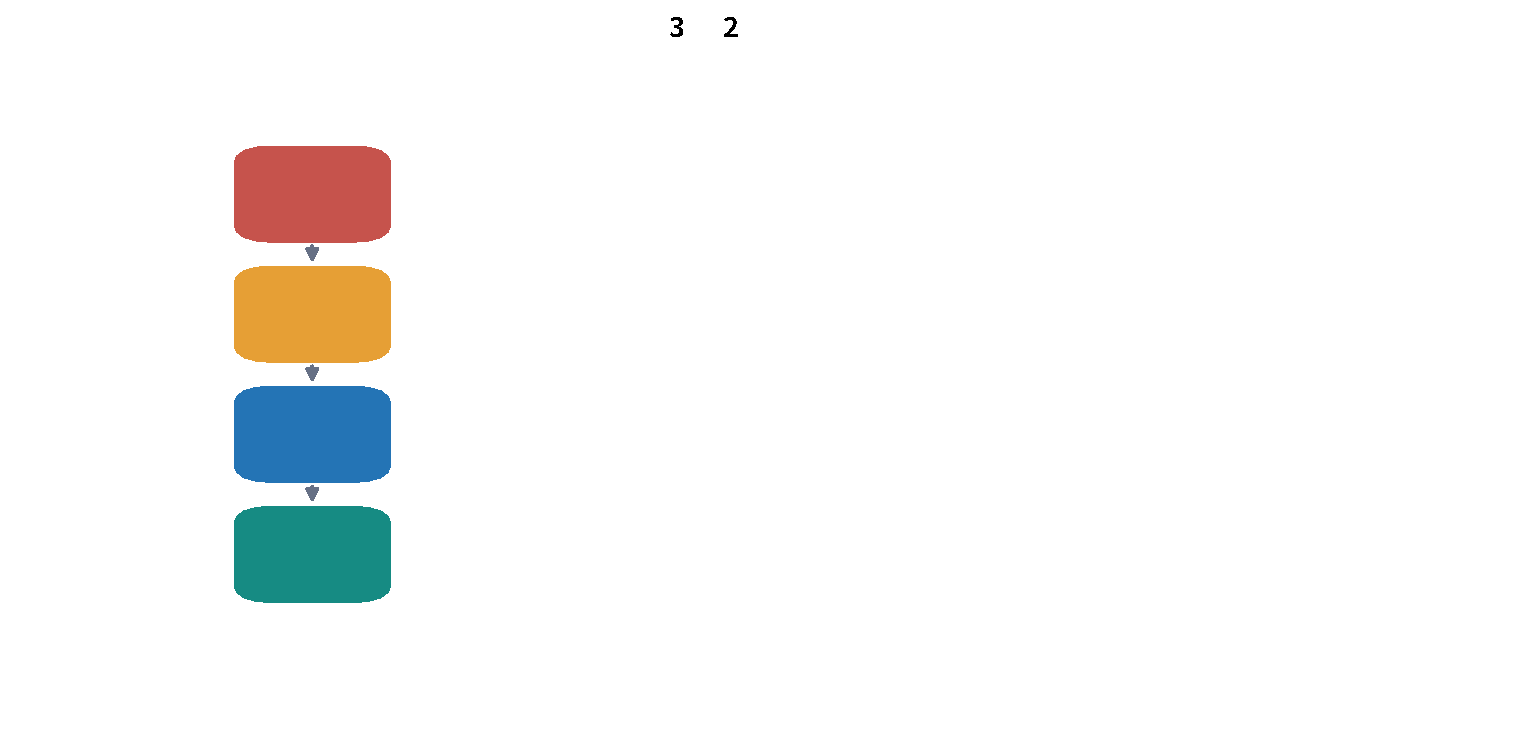
\includegraphics[width=.97\textwidth]{next_year_roadmap.pdf}
  \caption{未来一年优先级路线。先建立可复核评测，再强化基础模型与条件判断，随后验证强化学习增益，最终推进需要毫米级定位和接触控制的插管清洗。}
\end{figure}

\section{P0：解除当前阻塞——让结果可信}

\begingroup\small\setlength{\tabcolsep}{2pt}
\begin{longtable}{>{\bfseries\raggedright\arraybackslash}p{16mm}>{\raggedright\arraybackslash}p{25mm}>{\raggedright\arraybackslash}p{36mm}>{\raggedright\arraybackslash}p{31mm}>{\raggedright\arraybackslash}p{28mm}}
\caption{P0 工作包}\\
\toprule
目标 & 操作 & 验证指标 & 前置条件/风险 & 预计产出\\
\midrule\endfirsthead
\toprule
目标 & 操作 & 验证指标 & 前置条件/风险 & 预计产出\\
\midrule\endhead
固定测试协议 &
规定瓶型、数量、姿态、密度、光照、回收盒位置和每组重复次数 &
每次测试都有场景编号、起止时间、逐瓶结果和异常原因 &
需冻结一批不进入训练的数据；避免测试过程中继续改规则 &
标准测试手册与不可变测试清单\\
\addlinespace
成功判定 &
分别记录抓瓶、抓盖、稳定瓶身、旋转、完全脱离、瓶/盖进正确盒 &
各阶段自动/人工一致率；完整任务成功率与95\%置信区间 &
仅靠一名观察者可能有偏差；需要双人复核或视频复核 &
阶段化结果表与自动统计面板\\
\addlinespace
运行记录 &
为每轮任务记录时间、模型版本、数据版本、瓶子编号、结果和恢复 &
零缺失记录；每次展示可追溯到保存模型与测试场景 &
注意隐私和设备信息脱敏 &
统一实验台账与日报\\
\addlinespace
端到端性能 &
记录推理延迟、控制丢帧、动作片段切换和设备中止 &
延迟 p50/p95/p99、控制频率、切换跳变和中止次数 &
测量工具本身不能影响实时运行 &
性能基准与告警阈值\\
\bottomrule
\end{longtable}
\endgroup

\section{P1：提高基础模型成功率}

\begingroup\small\setlength{\tabcolsep}{2pt}
\begin{longtable}{>{\bfseries\raggedright\arraybackslash}p{16mm}>{\raggedright\arraybackslash}p{25mm}>{\raggedright\arraybackslash}p{36mm}>{\raggedright\arraybackslash}p{31mm}>{\raggedright\arraybackslash}p{28mm}}
\caption{P1 工作包}\\
\toprule
目标 & 操作 & 验证指标 & 前置条件/风险 & 预计产出\\
\midrule\endfirsthead
\toprule
目标 & 操作 & 验证指标 & 前置条件/风险 & 预计产出\\
\midrule\endhead
修复空拧 &
采集同瓶型有盖/无盖配对轨迹；无盖明确要求跳过旋拧；加入判断阶段 &
无盖误进入旋拧率；有盖漏拧率；完整任务成功率 &
条件指令必须与实际动作一致；防止模型只记瓶型 &
无盖条件数据版本与对照报告\\
\addlinespace
修复倒抓 &
按瓶口方向和可抓取面分层采集；增加抓取后朝向确认和重新抓取 &
倒抓率、抓取后可旋盖率、重新抓取成功率 &
需要逐帧朝向/抓取端标签；避免只增加同一方向样本 &
方向平衡数据与抓取诊断表\\
\addlinespace
提高接触稳定性 &
分开标注接近、夹盖、转动、脱离；记录夹爪电流与视觉瓶盖角 &
抓盖率、开始转动率、完全脱离率、掉落率 &
瓶盖类型和摩擦差异大；视觉角度估计需标定 &
接触阶段数据集与阶段模型对比\\
\addlinespace
优化动作片段 &
比较不同执行长度、重规划时刻和异常打断策略 &
完成时间、切换跳变、失败后恢复率、控制丢帧 &
不能同时改变数据和模型，以免无法归因 &
动作片段消融报告\\
\addlinespace
增加多视角鲁棒性 &
在不改变其他条件下比较顶部、腕部缺失或遮挡 &
三相机消融下的阶段完成率和动作偏差 &
注意力不能替代遮挡实验；需保证安全 &
相机贡献报告与最小传感器配置\\
\bottomrule
\end{longtable}
\endgroup

\section{P2：建立可靠比较并推进强化学习}

强化学习应建立在可用的基础模型和统一测试协议上。下一年度先冻结一个基础模型版本，再在同一数据、同一瓶子、同一初始条件和同一测试次数下比较基础模型与强化学习模型。

\begingroup\small\setlength{\tabcolsep}{2pt}
\begin{longtable}{>{\bfseries\raggedright\arraybackslash}p{16mm}>{\raggedright\arraybackslash}p{25mm}>{\raggedright\arraybackslash}p{36mm}>{\raggedright\arraybackslash}p{31mm}>{\raggedright\arraybackslash}p{28mm}}
\caption{P2 工作包}\\
\toprule
目标 & 操作 & 验证指标 & 前置条件/风险 & 预计产出\\
\midrule\endfirsthead
\toprule
目标 & 操作 & 验证指标 & 前置条件/风险 & 预计产出\\
\midrule\endhead
同条件基础对照 &
冻结基础模型和测试集；强化学习只改变一个因素 &
完整任务与各阶段成功率差值、置信区间、耗时与碰撞 &
基础模型仍快速变化会使对照失效 &
可复核基础模型基线\\
\addlinespace
改进奖励 &
把人工终止标签拆为阶段奖励，检查重复/错误标签 &
标签一致率、价值判断校准、离线排序正确率 &
错误奖励会放大错误行为 &
奖励规范与清洗数据\\
\addlinespace
多随机种子 &
至少 3 个随机种子重复关键配置 &
均值、标准差和95\%置信区间 &
计算成本高，应先缩小候选配置 &
多种子实验表\\
\addlinespace
安全真机验证 &
先离线筛选，再小批量真机；设置动作边界和人工急停 &
相对基础模型的阶段增益、异常次数与恢复率 &
真机探索存在碰撞和设备磨损风险 &
强化学习真机评估报告\\
\bottomrule
\end{longtable}
\endgroup

\section{P3：推进空瓶插入水管清洗}

未来一年计划把空瓶瓶口插入水管进行清洗。该任务比拧盖更依赖精确的瓶口中心、管口中心、轴线方向和接触顺应。当前“毫米级”是工程目标，不是已经测得的系统精度。

\begingroup\small\setlength{\tabcolsep}{2pt}
\begin{longtable}{>{\bfseries\raggedright\arraybackslash}p{16mm}>{\raggedright\arraybackslash}p{25mm}>{\raggedright\arraybackslash}p{36mm}>{\raggedright\arraybackslash}p{31mm}>{\raggedright\arraybackslash}p{28mm}}
\caption{P3 工作包}\\
\toprule
目标 & 操作 & 验证指标 & 前置条件/风险 & 预计产出\\
\midrule\endfirsthead
\toprule
目标 & 操作 & 验证指标 & 前置条件/风险 & 预计产出\\
\midrule\endhead
真实几何标定 &
测量瓶口、管口、相机和机器人坐标；记录重复定位误差 &
位置/角度误差均值、95分位和重复性 &
不同瓶型尺寸变化；标定漂移 &
几何基准与误差预算\\
\addlinespace
数字孪生 &
建立瓶子、水管、工作台和双臂碰撞模型；冻结审核场景 &
真实照片/测量对齐误差、碰撞一致率、轨迹可执行率 &
仿真外观相似不等于接触真实 &
可复核数字孪生场景\\
\addlinespace
分阶段插入 &
先定位，再对轴，再接触，再小距离插入，最后完成清洗 &
各阶段成功率、最大接触力、插入深度和完成时间 &
无力觉时应采用保守速度和视觉反馈 &
分阶段插入策略与安全规范\\
\addlinespace
数据与强化学习 &
采集毫米级失败边界与恢复；在安全仿真/离线数据中先优化 &
相对基础模仿模型的插入误差、恢复率和真机增益 &
仿真到真实差距；奖励设计可能诱导危险动作 &
插管数据集、对照实验和研究论文材料\\
\bottomrule
\end{longtable}
\endgroup

\section{未来一年验收主线}

未来一年不以“训练了更多步”作为验收，而以以下可复核结果为主线：

\begin{enumerate}
  \item 任何模型都能在固定测试集上给出完整任务和分阶段结果；
  \item 空拧和倒抓都有条件化错误率，并能被数据/方法修改显著降低；
  \item 基础模仿模型与强化学习模型有同条件、多随机种子比较；
  \item 插管任务有真实几何误差预算、分阶段指标和安全测试；
  \item 每一张结果图都能回到原始数据、模型版本和测试记录。
\end{enumerate}

\appendix
\chapter{配置与证据索引}

\section{机器与数据职责地图}

\begin{table}[H]
\centering
\caption{三类计算环境的职责}
\begin{tabularx}{\textwidth}{>{\bfseries}p{34mm}p{42mm}X}
\toprule
环境 & 主要职责 & 本报告使用方式\\
\midrule
数据中心机器 & 保存、编辑和发布各类机器人数据；运行数据编辑中心 & 只读核验有效 ALOHA 项目、轨迹、帧数、时长和平台功能\\
ALOHA 训练机器 & 主要训练仓库、历史版本、正式保存模型、采集软件和机器人运行 & 只读核验正式模型、训练历史、运行入口、注意力记录和采集能力；未启动机器人\\
本地研究机器 & 强化学习、数字孪生、离线分析与报告生成 & 读取现有研究产物；只在报告输出目录新增和修改文件\\
\bottomrule
\end{tabularx}
\end{table}

\section{核心数据字段}

\begin{table}[H]
\centering
\caption{基础模仿学习数据字段}
\begin{tabularx}{\textwidth}{>{\bfseries}p{35mm}p{32mm}X}
\toprule
字段 & 形状/类型 & 含义\\
\midrule
顶部画面 & 视频帧 & 整体工作台与双臂\\
左腕画面 & 视频帧 & 左夹爪和瓶身近景\\
右腕画面 & 视频帧 & 右夹爪和瓶口近景\\
底部画面 & 视频帧 & 原始数据保存，但正式模型未使用\\
机器人状态 & 14维连续量 & 左右臂关节与夹爪位置\\
动作 & 14维连续量 & 下一控制时刻的双臂关节与夹爪目标\\
任务文字 & 字符串 & 当前轨迹的任务描述\\
时间戳/帧号 & 数值 & 检查顺序、同步与轨迹长度\\
\bottomrule
\end{tabularx}
\end{table}

\section{重要证据编号}

\begin{longtable}{>{\bfseries}p{17mm}p{43mm}p{70mm}}
\caption{正文结论—证据索引（公开版）}\\
\toprule
编号 & 证据类型 & 支持内容\\
\midrule\endfirsthead
\toprule
编号 & 证据类型 & 支持内容\\
\midrule\endhead
E01 & 现场任务说明与运行配置 & 左取瓶、右旋盖、瓶/盖分箱的完整任务\\
E02 & 采集软件当前版本与历史 & 连续采集、重采、异步保存、触发、健康检查与停止能力\\
E03 & 数据中心项目与轨迹数据库 & 51个有效项目、2,413条轨迹、2,907,804帧、约16.15小时\\
E04 & 固定版本公开数据元数据 & 25个唯一仓库、1,051条轨迹、879,852帧及字段一致性\\
E05 & 全量数值数据检查 & 非有限值、全零行、时间戳、帧号与完全重复轨迹检查\\
E06 & 正式训练配置与模型结构 & 三路输入、14维状态/动作、50步动作片段与实际训练目标\\
E07 & 现场部署配置与控制流程 & 50Hz控制、后台重规划、动作限制与夹爪保护\\
E08 & 原始训练历史 & 6,059条记录、0--59,990步、约51.4小时与损失曲线\\
E09 & 正式保存模型元数据 & 第19,000步部署目录、8.38亿参数、归一化统计与可读取性\\
E10 & 现场观测声明 & 完整循环、超过1小时和约2瓶/分钟估计；同时声明缺失录像与计数\\
E11 & 数据条件与任务指令交叉检查 & 无盖、方向、翻转等条件规模及无盖指令缺口\\
E12 & 真实注意力运行清单 & 9份清单、8,223个样本、三路相机份额和解释边界\\
E13 & 训练平台运行谱系 & 41次尝试、14组配置、运行状态和达到步数的漏斗\\
E14 & 正式设备照片 & ALOHA示教臂、工作臂、相机与工作区；静止休眠状态\\
E15 & 强化学习数据统计 & 835条冲洗轨迹、裁剪帧、238,816个训练片段和人工奖励\\
E16 & 强化学习保存模型与轮次日志 & 6,154万参数、轮次28--32和离线验证动作误差\\
\bottomrule
\end{longtable}

更细的证据文件、字段、内部位置与可信度保存在报告目录的审计材料中，不在面向验收专家的正文中展示。

\section{关键数字复核表}

\begin{longtable}{>{\bfseries}p{50mm}p{28mm}p{47mm}}
\caption{报告关键数字及其口径}\\
\toprule
数字 & 值 & 口径\\
\midrule\endfirsthead
\toprule
数字 & 值 & 口径\\
\midrule\endhead
数据中心有效 ALOHA 数据 & 2,413条 / 16.15小时 & 51个有效项目，不含项目外562条\\
正式模型唯一训练数据 & 1,051条 / 4.89小时 & 25个唯一固定版本数据仓库\\
过滤后可训练数据 & 844,102帧 / 4.69小时 & 按50帧/秒换算\\
正式模型采样暴露 & 1,495条轨迹等效量 & 重复采样，不是新增轨迹\\
正式保存模型参数 & 838,358,468 & 仅模型参数；无优化器状态\\
正式训练历史 & 6,059条 / 59,990步 & 约51.4小时；现场部署19,000步\\
训练试验记录 & 41次 / 14组配置 & 运行尝试，不是成功实验数\\
真实注意力样本 & 8,223 & 9份运行清单；无结果标签\\
现场连续运行 & $>1$小时（估计） & 无完整录像、计数表或测试协议\\
现场平均处理速度 & 约2瓶/分钟（估计） & 不可计算置信区间\\
强化学习数据 & 835条 / 238,816片段 & 冲洗任务研究数据，与基础分拣数据分开\\
强化学习离线改善 & 约6.7\% & 固定验证动作误差；不是真机成功率\\
\bottomrule
\end{longtable}

\section{软件与环境摘要}

\begin{table}[H]
\centering
\caption{经审计的软件环境摘要}
\begin{tabularx}{\textwidth}{>{\bfseries}p{33mm}p{35mm}X}
\toprule
类别 & 版本/状态 & 说明\\
\midrule
Python & 3.11.14 & ALOHA 训练机器环境\\
JAX / JAXLIB & 0.5.3 / 0.5.3 & 基础模型训练与推理\\
PyTorch & 2.7.1 & 部分数据和强化学习工具\\
Flax / Orbax / Optax & 0.10.2 / 0.11.13 / 0.2.4 & 模型、保存与优化\\
OpenCV / LeRobot & 4.11.0.86 / 0.4.2 & 图像与机器人数据\\
Docker & 29.0.2 & 服务运行环境\\
ROS / Isaac Sim & 该指标尚未记录 & 本报告不以仿真或ROS运行作为完成证据\\
\bottomrule
\end{tabularx}
\end{table}

\section{缺失信息摘要}

\begin{longtable}{>{\bfseries}p{18mm}p{40mm}p{65mm}}
\caption{需要补充的关键证据}\\
\toprule
优先级 & 缺失内容 & 补充方法\\
\midrule\endfirsthead
\toprule
优先级 & 缺失内容 & 补充方法\\
\midrule\endhead
P0 & 正式逐瓶测试记录与完整录像 & 固定场景、逐次编号、同步录像、双人复核和不可变统计表\\
P0 & 自动任务与阶段判定 & 记录瓶盖存在/脱离、瓶身/瓶盖进盒和异常状态\\
P0 & 无盖/有盖与正反方向配对测试 & 同瓶型同位置成对测试，记录条件错误率\\
P1 & 保存点统一比较 & 冻结多个候选保存点，在同一测试集上评测\\
P1 & 视频全量解码与语义质量 & 全量解码校验，增加瓶盖存在性、方向和阶段标签\\
P1 & 接触量测 & 增加瓶盖角度、夹爪电流或力/触觉记录\\
P1 & 完整端到端延迟 & 记录推理、网络、动作切换和控制丢帧分布\\
P1 & 数据平台与公开数据网页视口截图 & 修复受审浏览器网关后，按登录后视口和公开数据网格分别截图\\
P2 & 多随机种子和独立测试集 & 至少3个随机种子，冻结未进入训练的测试场景\\
\bottomrule
\end{longtable}

\section{复现说明}

报告目录保存了机器可读数据统计、保存模型元数据、绘图原始表格、图形生成脚本、结论—证据矩阵和只读审计记录。统计与图形均可在不启动机器人、不修改远程数据的条件下重新生成。详细复现步骤写在随报告提供的 README 中。

\section{已知版式与媒体限制}

本报告遵守以下版式原则：图表标题直接给出主要信息；图下注明“这张图回答什么”和不可推导的结论；底层数据随报告保存；照片、训练示教、注意力和概念示意明确区分；不强制所有图片固定在原文位置，以减少半空白页；表格过长时自动跨页。数据可视化的可访问性和叙事性参考美国政府设计系统、英国政府统计图表清单和世界卫生组织数据设计语言\cite{uswds_dataviz,uk_chart_checklist,who_data_design}。

本报告没有完整演示视频，因此不设置视频展示页。数据中心和 Hugging Face 的浏览器视口截图因受审浏览器网关在编写期间不可用而没有纳入；报告使用真实数据库统计、固定版本公开数据和真实示教关键帧替代，但没有将其伪装成网页截图。



\bibliographystyle{plain}
\bibliography{bibliography/references}
\end{document}
